\Chapter{Bevezetés}

Dolgozatomban képként rendelkezésre álló kották adatainak automatizált módon történő feldolgozásával foglalkozom. A kinyert adatok további kezeléséhez, feldolgozásához szemantikus, konkrétan RDF keretrendszernek megfelel adatszervezési módot választottam. \Aref{fig:Dal1}. ábrán láthatunk egy példát egy feldolgozandó kottára.

\begin{figure}[h]
	\frame{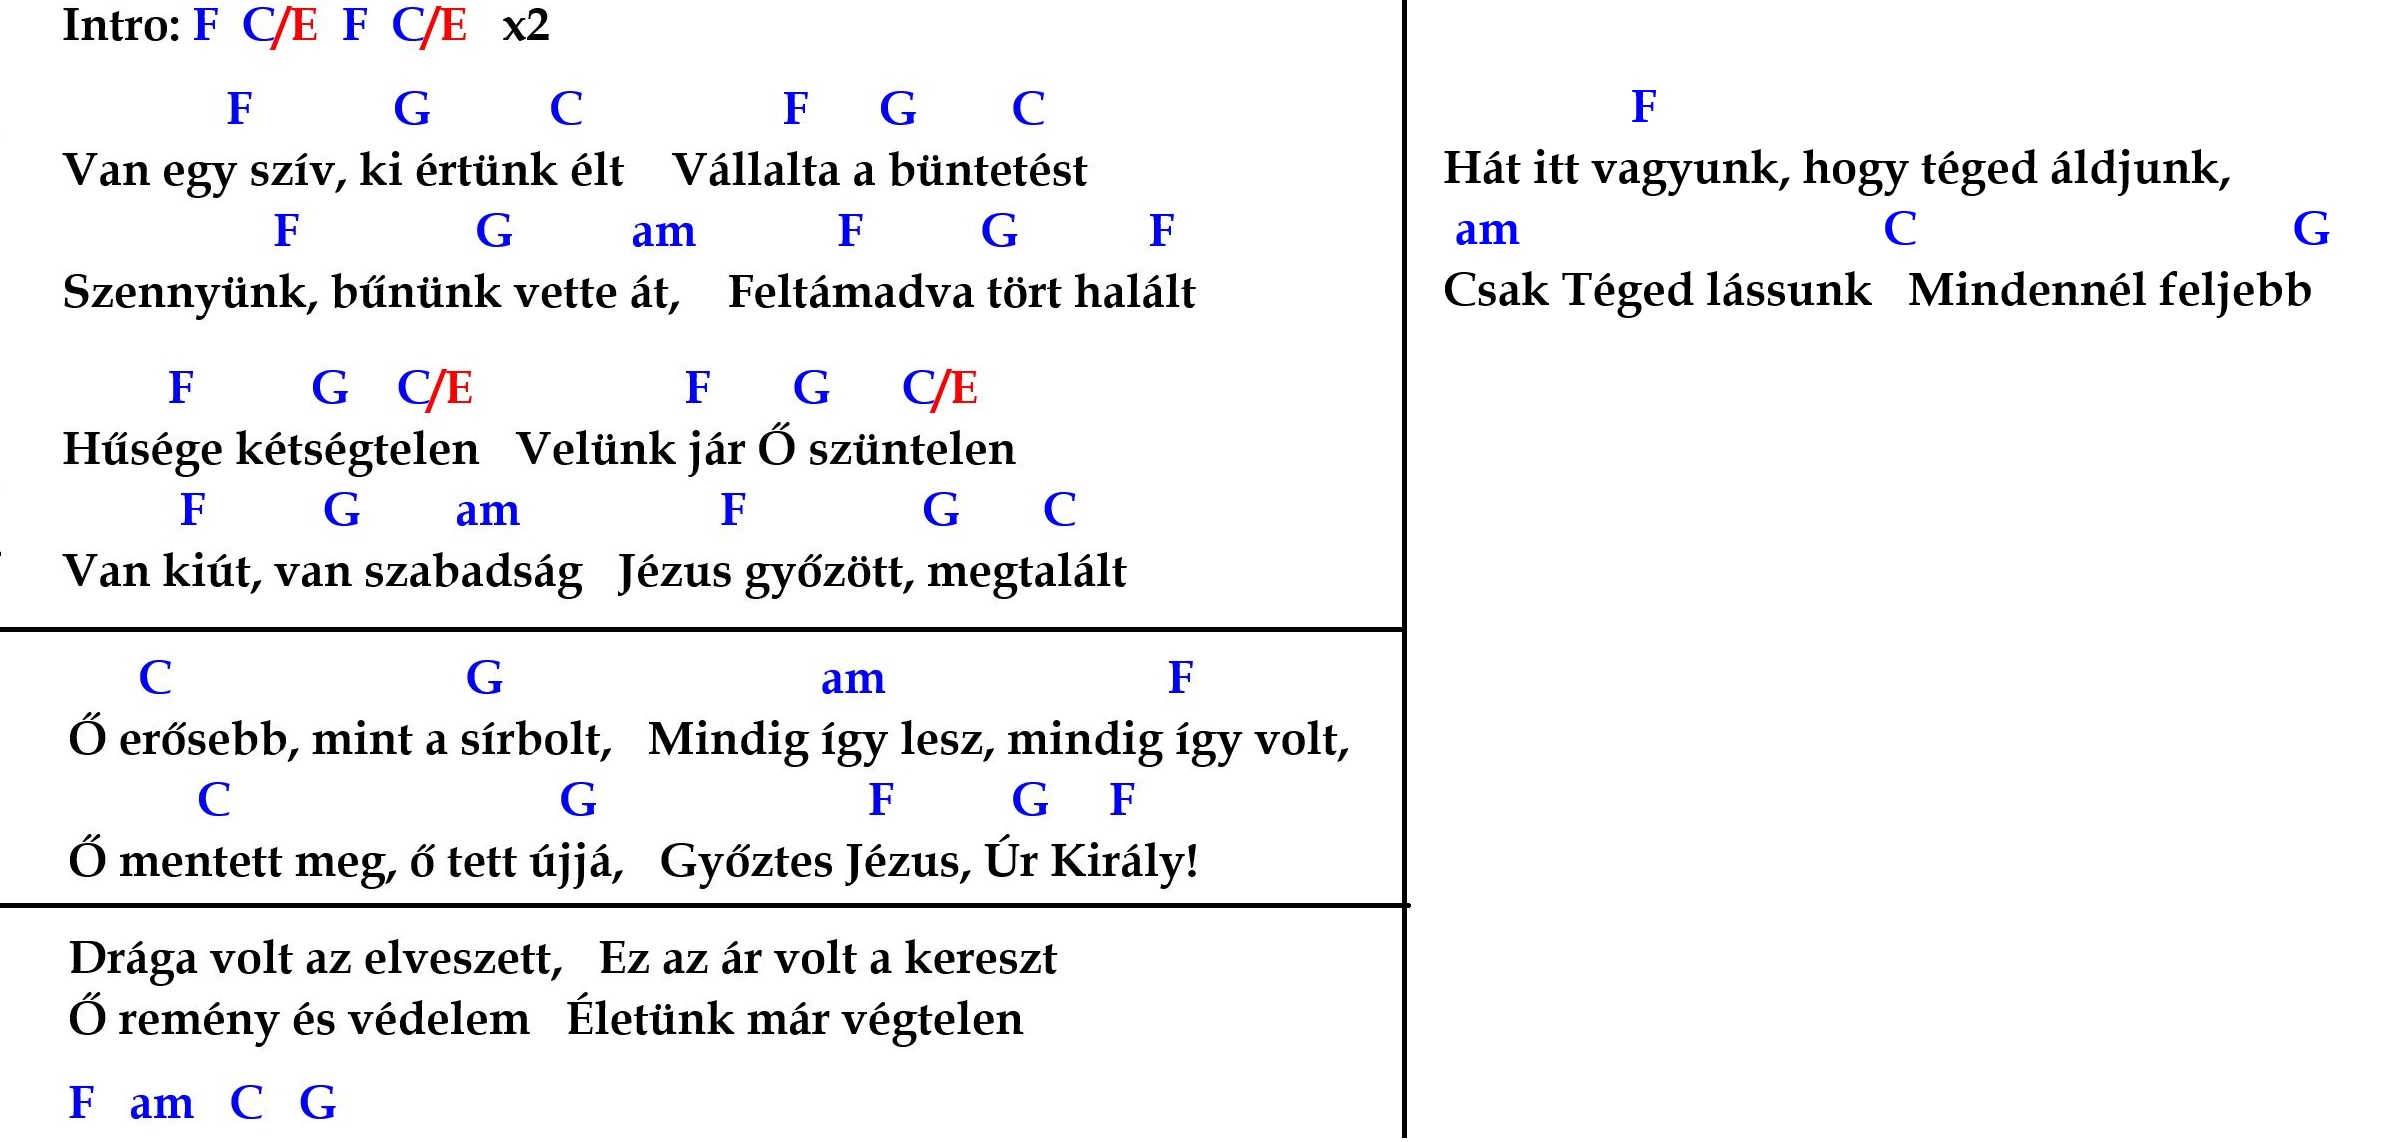
\includegraphics[width=\textwidth]{images/samples/O_erosebb.jpg}}
	\caption{"Ő erősebb" c. dal kottája.}
	\label{fig:Dal1}
\end{figure}

A dolgozat elkészítése során felépítettem a projektet és megismerkedtem a képfeldolgozás témakörével. Bevezetésképpen röviden áttekinteném a témához kötődő vizsgálatok és fejlesztések menetét.

Először csak egy kép beolvasására volt képes a programom, ezzel megnéztem, hogy milyen tulajdonságokkal rendelkezik maga az \textit{OpenCV} (\texttt{cv2}) programkönyvtár. Eljutottam addig, hogy a \textit{Tkinter} könyvtárral egy menüt létre tudjak hozni, amin 3 gomb van: előző kép, következő kép, és határérték változtatás névvel. Ugyanis a \texttt{cv2} programkönyvtárba sok lehetőség van arra, hogy egy képen egy objektumot meg tudjunk különböztetni. Jelenleg ami számomra célszerű volt az a kék színnek az elhatárolása, a szövegtől, hiszen a mintaadathalmazom kék színnel jelzi az akkordokat, amiket majd a programom ki fog venni szövegként, megváltoztatja, majd újra képpé alakítja azt.

Miután megismertem a \texttt{cv2}, számomra hasznos metódusait, ami jelenleg a kép beolvasása, szín szerinti elhatárolás, majd azon kép mutatása, elkezdtem foglalkozni azzal, hogy miként lehet szöveggé alakítani a képen látható betűket. Ehhez használom a \texttt{pytesseract} nevezetű programkönyvtárat. Azt teszi lehetővé, hogy egy beolvasott képből ki tudjam nyerni annak szöveget az \texttt{image\_to\_string} metódussal, így jelenleg a programom képes arra, hogy a képet (amit megkap paraméternek a metódus) átalakítsa szöveggé. Kezdetben az eredményeket csak a konzolra írattam ki, de később egy külön fájlba került mentésre.

Miután a program megállapítja, hogy ez milyen hangnemben van, az által, hogy milyen akkordok szerepelnek benne a legtöbbször, valamint, a kezdő akkord szerint. Ez az esetek egy részében megtévesztő lehet, mint például, hogy ha F-el kezdődik, miközben a dal C-dúrban van. Ezt követően a felhasználó kiválaszthatja, hogy milyen hangnembe szeretné lementeni a kottát, tegyük fel, hogy G-dúrba. Az előbbi példánál maradva a transzponálás során az F akkord-hármas C-re, a G D-re, a C G-re és az am em-ra fog változni. Ahhoz, hogy ez lementhető legyen, vissza kell illeszteni a megfelelő karaktereket a megfelelő színben a képhez. Ez a folyamat úgy fog kinézni, hogy a kiválasztott akkordok, mikor szöveggé alakulnak azután el is fognak tűnni a képről, és majd a visszaillesztésnél, a lementett koordináták szerint kerülnek vissza a megfelelő akkordok.

A dolgozatban a képfeldolgozás mellett a szemantikus adattárolási mód is nagy szerepet kap. A továbbiakban láthatjuk majd, hogy az adatok hogyan ábrázolhatók hármasok formájában, illetve hogy azokkal milyen további műveletek végezhetők el.
